\documentclass[journal,12pt,twocolumn]{IEEEtran}
\usepackage{setspace}
\usepackage{gensymb}
\usepackage{xcolor}
\usepackage{caption}
\singlespacing
\usepackage{siunitx}
\usepackage[cmex10]{amsmath}
\usepackage{mathtools}
\usepackage{hyperref}
\usepackage{amsthm}
\usepackage{mathrsfs}
\usepackage{txfonts}
\usepackage{stfloats}
\usepackage{cite}
\usepackage{cases}
\usepackage{subfig}
\usepackage{longtable}
\usepackage{multirow}
\usepackage{enumitem}
\usepackage{mathtools}
\usepackage{listings}
\usepackage{tikz}
\usetikzlibrary{shapes,arrows,positioning}
\usepackage{circuitikz}
\let\vec\mathbf
\DeclareMathOperator*{\Res}{Res}
\renewcommand\thesection{\arabic{section}}
\renewcommand\thesubsection{\thesection.\arabic{subsection}}
\renewcommand\thesubsubsection{\thesubsection.\arabic{subsubsection}}

\renewcommand\thesectiondis{\arabic{section}}
\renewcommand\thesubsectiondis{\thesectiondis.\arabic{subsection}}
\renewcommand\thesubsubsectiondis{\thesubsectiondis.\arabic{subsubsection}}
\hyphenation{op-tical net-works semi-conduc-tor}

\lstset{
language=Python,
frame=single, 
breaklines=true,
columns=fullflexible
}
\begin{document}
\theoremstyle{definition}
\newtheorem{theorem}{Theorem}[section]
\newtheorem{problem}{Problem}
\newtheorem{proposition}{Proposition}[section]
\newtheorem{lemma}{Lemma}[section]
\newtheorem{corollary}[theorem]{Corollary}
\newtheorem{example}{Example}[section]
\newtheorem{definition}{Definition}[section]
\newcommand{\BEQA}{\begin{eqnarray}}
\newcommand{\EEQA}{\end{eqnarray}}
\newcommand{\define}{\stackrel{\triangle}{=}}
\newcommand{\myvec}[1]{\ensuremath{\begin{pmatrix}#1\end{pmatrix}}}
\newcommand{\mydet}[1]{\ensuremath{\begin{vmatrix}#1\end{vmatrix}}}

\bibliographystyle{IEEEtran}
\providecommand{\nCr}[2]{\,^{#1}C_{#2}} % nCr
\providecommand{\nPr}[2]{\,^{#1}P_{#2}} % nPr
\providecommand{\mbf}{\mathbf}
\providecommand{\pr}[1]{\ensuremath{\Pr\left(#1\right)}}
\providecommand{\qfunc}[1]{\ensuremath{Q\left(#1\right)}}
\providecommand{\sbrak}[1]{\ensuremath{{}\left[#1\right]}}
\providecommand{\lsbrak}[1]{\ensuremath{{}\left[#1\right.}}
\providecommand{\rsbrak}[1]{\ensuremath{{}\left.#1\right]}}
\providecommand{\brak}[1]{\ensuremath{\left(#1\right)}}
\providecommand{\lbrak}[1]{\ensuremath{\left(#1\right.}}
\providecommand{\rbrak}[1]{\ensuremath{\left.#1\right)}}
\providecommand{\cbrak}[1]{\ensuremath{\left\{#1\right\}}}
\providecommand{\lcbrak}[1]{\ensuremath{\left\{#1\right.}}
\providecommand{\rcbrak}[1]{\ensuremath{\left.#1\right\}}}
\theoremstyle{remark}
\newtheorem{rem}{Remark}
\newcommand{\sgn}{\mathop{\mathrm{sgn}}}
\newcommand{\rect}{\mathop{\mathrm{rect}}}
\newcommand{\sinc}{\mathop{\mathrm{sinc}}}
\providecommand{\abs}[1]{\left\vert#1\right\vert}
\providecommand{\res}[1]{\Res\displaylimits_{#1}} 
\providecommand{\norm}[1]{\lVert#1\rVert}
\providecommand{\mtx}[1]{\mathbf{#1}}
\providecommand{\mean}[1]{E\left[ #1 \right]}
\providecommand{\fourier}{\overset{\mathcal{F}}{ \rightleftharpoons}}
\providecommand{\ztrans}{\overset{\mathcal{Z}}{ \rightleftharpoons}}
\providecommand{\system}[1]{\overset{\mathcal{#1}}{ \longleftrightarrow}}
\newcommand{\solution}{\noindent \textbf{Solution: }}
\providecommand{\dec}[2]{\ensuremath{\overset{#1}{\underset{#2}{\gtrless}}}}
\numberwithin{equation}{section}
\makeatletter
\@addtoreset{figure}{problem}
\makeatother
\let\StandardTheFigure\thefigure
\renewcommand{\thefigure}{\theproblem}
\def\putbox#1#2#3{\makebox[0in][l]{\makebox[#1][l]{}\raisebox{\baselineskip}[0in][0in]{\raisebox{#2}[0in][0in]{#3}}}}
     \def\rightbox#1{\makebox[0in][r]{#1}}
     \def\centbox#1{\makebox[0in]{#1}}
     \def\topbox#1{\raisebox{-\baselineskip}[0in][0in]{#1}}
     \def\midbox#1{\raisebox{-0.5\baselineskip}[0in][0in]{#1}}

\vspace{3cm}
\title{Fourier Series}
\author{Gautam Singh}
\maketitle
\tableofcontents
\renewcommand{\thefigure}{\theenumi}
\renewcommand{\thetable}{\theenumi}
\bigskip
\begin{abstract}
This manual provides a simple introduction to Fourier Series.
\end{abstract}
\section{Periodic Function}
Let 
\begin{align}
	x(t) &= A_0\abs{\sin\brak{2\pi f_0 t}}
	\label{eq:10-orig-diff-def}
\end{align}
\begin{enumerate}[label=\thesection.\arabic*
,ref=\thesection.\theenumi]
\item Plot $x(t)$.

\solution The Python code \texttt{codes/1\_1.py} plots $x(t)$ 
in Fig. \ref{fig:xt}.
\begin{figure}[!htp]
    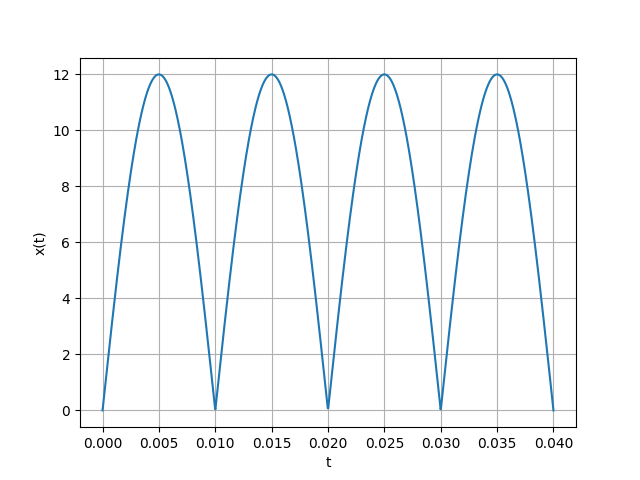
\includegraphics[width=\columnwidth]{figs/1_1.png}
    \caption{$x(t)$}
    \label{fig:xt}
\end{figure}
\item Show that $x(t)$ is periodic and find its period.

\solution Note that,
\begin{align}
    x\brak{t+\frac{1}{2f_0}} &= A_0\abs{\sin\brak{2\pi f_0\brak{t + \frac{1}{2f_0}}}} \\
                            &= A_0\abs{\sin\brak{2\pi f_0t + \pi}} \\
                            &= A_0\abs{\sin\brak{2\pi f_0t}}
\end{align}
Hence the period of $x(t)$ is $\frac{1}{2f_0}$.
\end{enumerate}
\section{Fourier Series}
Consider $A_0 =12$ and $f_0 = 50$ for all numerical calculations.
\begin{enumerate}[label=\thesection.\arabic*,ref=\thesection.\theenumi]
\item If
\begin{align}
	x(t) = \sum_{k = -\infty}^{\infty}c_ke^{\j2\pi kf_0 t}
\label{eq:one-Z-complex}
\end{align}
show that 
\begin{align}
	c_k = f_0\int_{-\frac{1}{2f_0}}^{\frac{1}{2f_0}}x(t)e^{-\j2\pi kf_0 t}\, dt
\label{eq:one-Z}
\end{align}

\solution For some $n \in \mathbb{Z}$,
\begin{align}
    x(t)e^{-\j2\pi nf_0t} = \sum_{k = -\infty}^{\infty}c_ke^{\j2\pi (k - n)f_0 t}
\end{align}
But
\begin{align}
    \int_{-\frac{1}{2f_0}}^{\frac{1}{2f_0}}e^{\j2\pi kf_0 t}\, dt = 
    \frac{1}{f_0}\delta_{0k}
\end{align}
where $\delta_{ij}$ denotes the Kronecker delta. Thus,
\begin{align}
    \int_{-\frac{1}{2f_0}}^{\frac{1}{2f_0}}x(t)e^{-\j2\pi nf_0 t}\, dt = 
    \frac{c_n}{f_0} \\
    \implies c_n = f_0\int_{-\frac{1}{2f_0}}^{\frac{1}{2f_0}}x(t)e^{-\j2\pi nf_0 t}\, dt 
\end{align}
\item Find $c_k$ for \eqref{eq:10-orig-diff-def}

\solution Using \eqref{eq:one-Z},
\begin{align}
    c_n &= f_0\int_{-\frac{1}{2f_0}}^{\frac{1}{2f_0}}A_0\abs{\sin\brak{2\pi f_0t}}
    e^{-\j2\pi nf_0t}\, dt \\
        &= f_0\int_{-\frac{1}{2f_0}}^{\frac{1}{2f_0}}A_0\abs{\sin\brak{2\pi f_0t}}
    \cos\brak{2\pi nf_0t}\, dt \nonumber \\
        &+ \j f_0\int_{-\frac{1}{2f_0}}^{\frac{1}{2f_0}}A_0
        \abs{\sin\brak{2\pi f_0t}}\sin\brak{2\pi nf_0t}\, dt \\
        &= 2f_0\int_{0}^{\frac{1}{2f_0}}A_0\sin\brak{2\pi f_0t}\cos\brak{2\pi nf_0t}\, dt \\
        &= f_0A_0\int_{0}^{\frac{1}{2f_0}}\brak{\sin\brak{2\pi\brak{n+1}f_0t}}\, dt \nonumber \\ 
        &- f_0A_0\int_{0}^{\frac{1}{2f_0}}\brak{\sin\brak{2\pi\brak{n-1}f_0t}}\, dt \\ 
        &= A_0\frac{1+\brak{-1}^n}{2\pi}\brak{\frac{1}{n+1} - \frac{1}{n-1}} \\
        &= 
        \begin{cases}
            \frac{2A_0}{\pi\brak{1-n^2}} & n\ \text{even} \\
            0 & n\ \text{odd}
        \end{cases}
        \label{eq:ck-xt}
\end{align}
\item Verify \eqref{eq:one-Z-complex} using python.

\solution The Python code \texttt{codes/2\_3.py} verifies \eqref{eq:one-Z-real}
by plotting Fig. \ref{fig:ver-complex}.
\begin{figure}[!ht]
    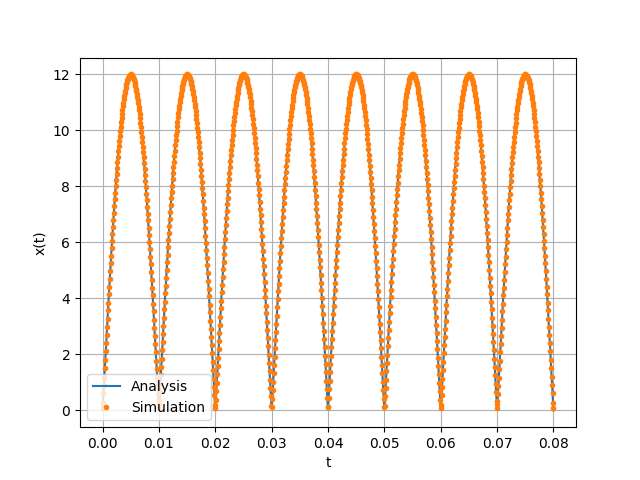
\includegraphics[width=\columnwidth]{figs/2_3.png}
    \caption{Verification of \eqref{eq:one-Z-complex}.}
    \label{fig:ver-complex}
\end{figure}

\item Show that 
\begin{align}
	x(t) = \sum_{k = 0}^{\infty}\brak{a_k\cos{\j2\pi kf_0 t}+b_k\sin{\j2\pi kf_0 t}}
\label{eq:one-Z-real}
\end{align}
and obtain the formulae for $a_k$ and $b_k$.

\solution From \eqref{eq:one-Z-complex},
\begin{align}
    x(t) &= \sum_{k = -\infty}^{\infty}c_ke^{\j2\pi kf_0 t} \\
         &= c_0 + \sum_{k = 1}^{\infty}c_ke^{\j2\pi kf_0t} + c_{-k}e^{-\j2\pi kf_0t} \\
         &= c_0 + \sum_{k = 1}^{\infty}\brak{c_k + c_{-k}}\cos\brak{2\pi kf_0t}  \nonumber \\
         &+ \sum_{k = 0}^{\infty}\j\brak{c_k - c_{-k}}\sin\brak{2\pi kf_0t}
\end{align}
Hence, for $k \ge 0$,
\begin{align}
    a_k &= 
    \begin{cases}
        c_0 & k = 0 \\
        c_k + c_{-k} & k > 0
    \end{cases} \label{eq:ak} \\
        &=
    \begin{cases}
        f_0\int_{-\frac{1}{2f_0}}^{\frac{1}{2f_0}}x(t)\, dt & k = 0 \\
        2f_0\int_{-\frac{1}{2f_0}}^{\frac{1}{2f_0}}
        x(t)\cos\brak{2\pi kf_0t}\, dt & k > 0
    \end{cases} \\
    b_k &= \frac{c_k - c_{-k}}{\j} = 2f_0\int_{-\frac{1}{2f_0}}^{\frac{1}{2f_0}}
    x(t)\sin\brak{2\pi kf_0t}\, dt
    \label{eq:bk}
\end{align}
\item Find $a_k$ and $b_k$ for 
	\eqref{eq:10-orig-diff-def}

\solution From \eqref{eq:one-Z-complex}, we see that since $x(t)$ is even,
\begin{align}
    x(-t) &= \sum_{k = -\infty}^{\infty}c_ke^{-\j2\pi kf_0 t} \\
          &= \sum_{k = -\infty}^{\infty}c_{-k}e^{\j2\pi kf_0t} \label{eq:sub} \\
          &= \sum_{k = -\infty}^{\infty}c_ke^{\j2\pi kf_0 t}
\end{align}
where we substitute $k := -k$ in \eqref{eq:sub}. Hence, we see that 
$c_k = c_{-k}$. So, from \eqref{eq:ak} and \eqref{eq:bk}, for $k \ge 0$,
\begin{align}
    a_k &= 
    \begin{cases}
        \frac{2A_0}{\pi} & k = 0 \\
        \frac{4A_0}{\pi\brak{1 - k^2}} & k > 0,\ k\ \text{even} \\
        0 & \text{otherwise}
    \end{cases} \label{eq:ak-xt}\\
    b_k &= 0
    \label{eq:bk-xt}
\end{align}
\item Verify 
\eqref{eq:one-Z-real}
using python.

\solution The Python code \texttt{codes/2\_6.py} verifies \eqref{eq:one-Z-real}
by plotting Fig. \ref{fig:ver-real}.
\begin{figure}[!ht]
    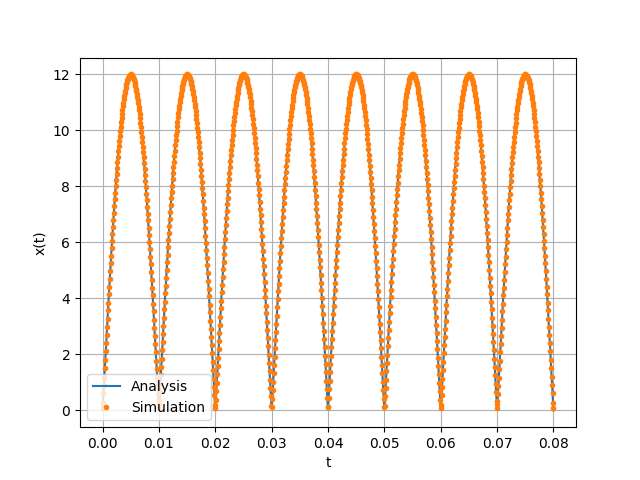
\includegraphics[width=\columnwidth]{figs/2_6.png}
    \caption{Verification of \eqref{eq:one-Z-real}.}
    \label{fig:ver-real}
\end{figure}
\end{enumerate}
\section{Fourier Transform}

\begin{enumerate}[label=\thesection.\arabic*
,ref=\thesection.\theenumi]
\item 
\begin{align}
	\delta(t)&=0, \quad t\neq 0 \\
	\int_{-\infty}^{\infty}\delta(t) \, dt&= 1
\end{align}
\item The Fourier Transform of $g(t)$ is
\begin{align}
G(f)=\int_{-\infty}^{\infty}g(t)e^{-j2\pi ft}\,dt
\label{eq:fourier}
\end{align}
\item Show that 
\begin{align}
    g(t-t_0)&\system{F}G(f)e^{-j2\pi ft_0}
    \label{eq:t-shift}
\end{align}

\solution We write, substituting $u := t-t_0$,
\begin{align}
    g(t-t_0)&\system{F}\int_{-\infty}^{\infty}
            g(t-t_0)e^{-\j2\pi ft}\,dt \\
            &=\int_{-\infty}^{\infty}
            g(u)e^{-\j2\pi f(u + t_0)}\,du \\
            &=G(f)e^{-j2\pi ft_0}
\end{align}
where the last equality follows from \eqref{eq:fourier}.
\item Show that
\begin{align}
    G(t)&\system{F}g(-f)
\end{align}

\solution Using the definition of the Inverse Fourier Transform,
\begin{align}
    g(t)=\int_{-\infty}^{\infty}G(f)e^{\j2\pi ft}\,df
    \label{eq:duality}
\end{align}
Hence, setting $t := -f$ and $f := t$, which implies $df = dt$,
\begin{align}
    g(-f)&=\int_{-\infty}^{\infty}G(t)e^{-\j2\pi ft}\,dt \\
    \implies G(t)&\system{F}g(-f)
\end{align}
\item $\delta(t)\system{F}?$

\solution We have, from the definition of $\delta(t)$,
\begin{align}
    \delta(t)&\system{F}\int_{-\infty}^{\infty}\delta(t)e^{-\j2\pi ft}\, dt \\
             &=\int_{-\infty}^{\infty}\delta(0)\, dt \\
             &=\int_{-\infty}^{\infty}\delta(t)\, dt = 1
             \label{eq:fourier-delta}
\end{align}
\item $e^{-j2\pi f_0t}\system{F}?$

\solution Suppose $g(t)\system{F}G(f)$. Then,
\begin{align}
    g(t)e^{\j2\pi f_0t}&\system{F}\int_{-\infty}^{\infty}
                       g(t)e^{-\j2\pi\brak{f-f_0}t}\, dt \\
                       &=F(f-f_0)
                       \label{eq:f-shift}
\end{align}
Using \eqref{eq:duality} in \eqref{eq:fourier-delta}, $1\system{F}\delta(-f)$.
Hence, applying \eqref{eq:f-shift},
\begin{align}
    e^{-\j2\pi f_0t}\system{F}\delta(-(f+f_0)) = \delta(f+f_0)
    \label{eq:fourier-exp}
\end{align}
\item $\cos(2\pi f_0t)\system{F}?$

\solution Using the linearity of the Fourier 
Transform and \eqref{eq:fourier-exp},
\begin{align}
    \cos\brak{2\pi f_0t} &= \frac{1}{2}
                         \brak{e^{\j2\pi f_0t} + e^{-\j2\pi f_0t}} \\
                         &\system{F}\frac{1}{2}\brak{\delta\brak{f+f_0} + \delta\brak{f-f_0}}
\end{align}
\item Find the Fourier Transform of $x(t)$ and plot it. Verify using python.

\solution Substituting \eqref{eq:ck-xt} in \eqref{eq:one-Z-complex},
\begin{align}
    x(t)&\system{F}\sum_{k=-\infty}^{\infty}c_k\delta\brak{f+kf_0} \\
        &=\frac{2A_0}{\pi}\sum_{k=-\infty}^{\infty}\frac{\delta\brak{f+2kf_0}}{1-4k^2}
        \label{eq:fourier-xt}
\end{align}
The python code \texttt{codes/3\_8.py} verifies \eqref{eq:fourier-xt}
while plotting Fig. \ref{fig:fourier-xt}
\begin{figure}[!ht]
    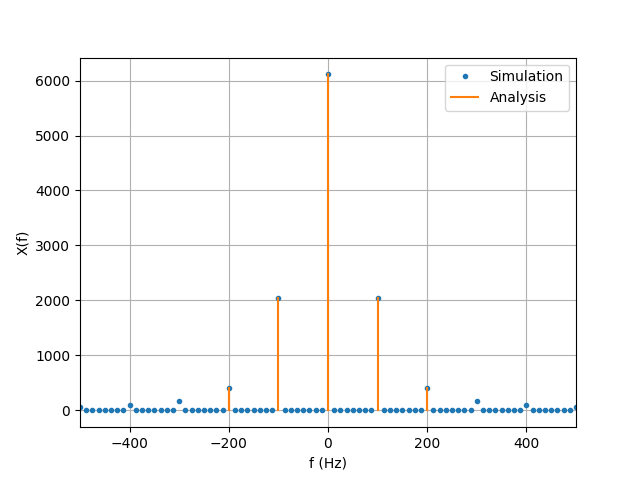
\includegraphics[width=\columnwidth]{figs/3_8.png}
    \caption{Fourier Transform of $x(t)$.}
    \label{fig:fourier-xt}
\end{figure}
\item Show that
\begin{align}
    \rect{t} \system{F} \sinc{f}
\end{align}
Verify using python.

\solution We write
\begin{align}
    \rect{t}&\system{F}\int_{-\infty}^{\infty}\rect{t}e^{-\j2\pi ft}\, dt \\
            &=\int_{-\frac{1}{2}}^{\frac{1}{2}}e^{-\j2\pi ft}\, dt \\
            &=\frac{e^{\j\pi f} - e^{-\j\pi f}}{\j2\pi f} = \frac{\sin{\pi f}}{\pi f} = \sinc{f}
            \label{eq:fourier-rect}
\end{align}
The python code \texttt{codes/3\_9.py} verifies \eqref{eq:fourier-rect}
by plotting Fig. \ref{fig:fourier-rect}.
\begin{figure}[!ht]
    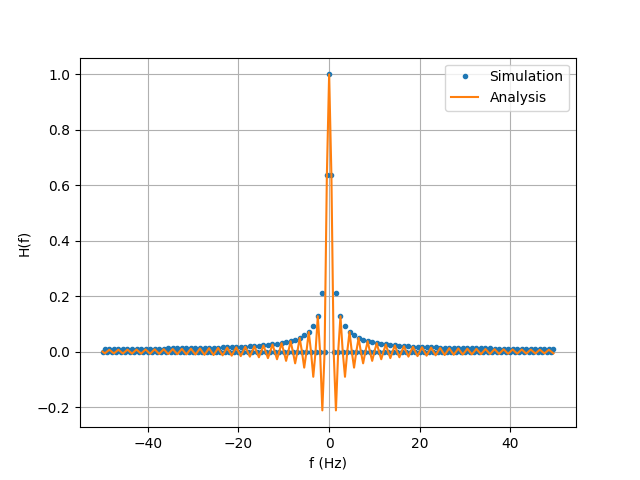
\includegraphics[width=\columnwidth]{figs/3_9.png}
    \caption{Fourier Transform of $\rect(t)$.}
    \label{fig:fourier-rect}
\end{figure}
\item $\sinc{t}\system{F} ?$  Verify using python.

\solution From \eqref{eq:duality}, we have 
\begin{align}
    \sinc{t}\system{F}\rect(-f)=\rect{f}
    \label{eq:fourier-sinc}
\end{align}
Since $\rect{f}$ is an even function.
The python code \texttt{codes/3\_10.py} verifies \eqref{eq:fourier-sinc}
by plotting Fig. \ref{fig:fourier-sinc}.
\begin{figure}[!ht]
    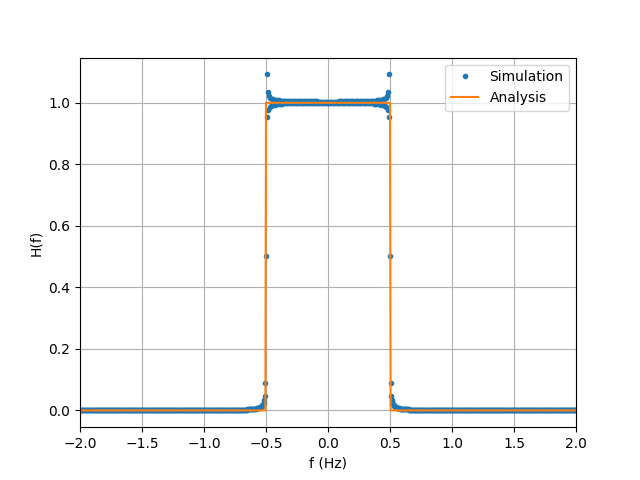
\includegraphics[width=\columnwidth]{figs/3_10.png}
    \caption{Fourier Transform of $\sinc(t)$.}
    \label{fig:fourier-sinc}
\end{figure}
\end{enumerate}

\section{Filter}
\begin{enumerate}[label=\thesection.\arabic*
,ref=\thesection.\theenumi]
\item Find $H(f)$ which transforms $x(t)$ to DC 5V.

\solution The function $H(f)$ is a low pass filter which filters out
even harmonics and leaves the zero frequency component behind.
The rectangular function represents an ideal low pass filter. 
Suppose the cutoff frequency is $f_c = 50$ Hz, then
\begin{align}
    H(f) = \rect{\frac{f}{2f_c}} =
    \begin{cases}
        1 & \abs{f} < f_c \\
        0 & \textrm{otherwise}
    \end{cases}
    \label{eq:Hf}
\end{align}
Multiplying by a scaling factor to get DC 5V,
\begin{align}
    H(f) = \frac{\pi V_0}{2A_0}\rect{\brak{\frac{f}{2f_c}}}
\end{align}
where $V_0 = 5$ V.
\item Find $h(t)$.

\solution Suppose $g(t)\system{F}G(f)$. Then, for some
nonzero $a \in \mathbb{R}$
\begin{align}
    g(at)&\system{F}\int_{-\infty}^{\infty}g(at)e^{-\j2\pi ft}\, dt \\
         &=\frac{1}{a}\int_{-\infty}^{\infty}g(u)e^{\brak{-\j2\pi \frac{f}{a}t}}\, dt \\
         &=\frac{1}{a}G\brak{\frac{f}{a}}
         \label{eq:t-scaling}
\end{align}
where we have substituted $u := at$. Using 
\eqref{eq:t-scaling} of the Fourier Transform in \eqref{eq:Hf},
\begin{align}
    h(t) = \frac{2\pi V_0}{A_0}f_c\sinc\brak{2f_ct}
\end{align}
\item Verify your result using convolution.

\solution The Python code \texttt{codes/4\_3.py} verifies the result
by plotting the graph below.
\begin{figure}[!ht]
    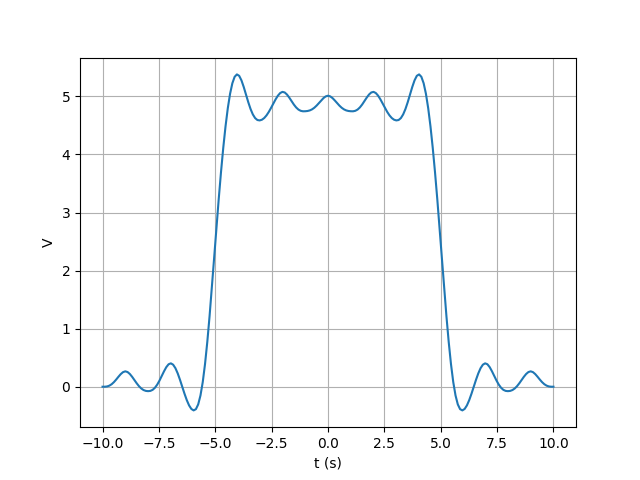
\includegraphics[width=\columnwidth]{figs/4_3.png}
    \caption{Convolution of the two signals.}
    \label{eq:fig-conv}
\end{figure}
\end{enumerate}
\section{Filter Design}
\begin{enumerate}[label=\thesection.\arabic*
,ref=\thesection.\theenumi]
\item Design a Butterworth filter for $H(f)$.

\solution The Butterworth filter has an amplitude response
given by
\begin{align}
    \abs{H\brak{f}}^2 = \frac{1}{\brak{1 + \brak{\frac{f}{f_c}}^{2n}}}
\end{align}
where $n$ is the order of the filter and $f_c$ is the cutoff
frequency. The attenuation at frequency $f$ is given by 
\begin{align}
    A &= -10\log_{10}\abs{H\brak{f}}^2 \\
      &= -20\log_{10}\abs{H\brak{f}}
    \label{eq:loss}
\end{align}
We consider the following design parameters for our
lowpass analog Butterworth filter:
\begin{enumerate}
    \item Passband edge, $f_p = 50$ Hz
    \item Stopband edge, $f_s = 100$ Hz
    \item Passband attenuation, $A_p = -1$ dB
    \item Stopband attenuation, $A_s = -20$ dB
\end{enumerate}
We are required to find a desriable order $n$ and cutoff
frequency $f_c$ for the filter. From \eqref{eq:loss},
\begin{align}
    A_p &= -10\log_{10}\sbrak{1 + \brak{\frac{f_p}{f_c}}^{2n}} \\
    A_s &= -10\log_{10}\sbrak{1 + \brak{\frac{f_s}{f_c}}^{2n}}
\end{align}
Thus,
\begin{align}
    \brak{\frac{f_p}{f_c}}^{2n} = 10^{-\frac{A_p}{10}} - 1 \label{eq:fc1} \\
    \brak{\frac{f_s}{f_c}}^{2n} = 10^{-\frac{A_s}{10}} - 1 \label{eq:fc2}
\end{align}
Therefore, on dividing the above equations and solving for $n$,
\begin{align}
    n = \frac{\log\brak{10^{-\frac{A_s}{10}} - 1} - 
    \log\brak{10^{-\frac{A_p}{10}} - 1}}{2\brak{\log{f_s} - \log{f_p}}}
\end{align}
In this case, making appropriate susbstitutions gives $n = 4.29$.
Hence, we take $n = 5$. Solving for $f_c$ in \eqref{eq:fc1} and
\eqref{eq:fc2},
\begin{align}
    f_{c1} = f_p\sbrak{10^{-\frac{A_p}{10}} - 1}^{-\frac{1}{2n}} = \SI[parse-numbers=false]{57.23}{\hertz} \\
    f_{c2} = f_s\sbrak{10^{-\frac{A_s}{10}} - 1}^{-\frac{1}{2n}} = \SI[parse-numbers=false]{63.16}{\hertz}
\end{align}
Hence, we take $f_c = \sqrt{f_{c1}f_{c2}} = \SI[parse-numbers=false]{60}{\hertz}$ approximately.

\item Design a Chebyshev filter for $H(f)$.

\solution The Chebyshev filter has an amplitude response
given by
\begin{align}
    \abs{H\brak{f}}^2 = \frac{1}{\brak{1 + \epsilon^2C_n^2\brak{\frac{f}{f_c}}}}
\end{align}
where 
\begin{enumerate}
    \item $n$ is the order of the filter
    \item $\epsilon$ is the ripple
    \item $f_c$ is the cutoff frequency 
    \item $C_n = \cosh^{-1}\brak{n\cosh{x}}$ denotes 
    the n\textsuperscript{th} order Chebyshev polynomial,
    given by
    \begin{align}
        c_n(x) =
        \begin{cases}
            \cos\brak{n\cos^{-1}x} & \abs{x} \le 1 \\
            \cosh\brak{n\cosh^{-1}x} & \textrm{otherwise}
        \end{cases}
        \label{eq:chebypol}
    \end{align}
\end{enumerate}
We are given the following specifications:
\begin{enumerate}
    \item Passband edge (which is equal to 
    cutoff frequency), $f_p = f_c$
    \item Stopband edge, $f_s$
    \item Attenuation at stopband edge, $A_s$
    \item Peak-to-peak ripple $\delta$ in the passband.
    It is given in dB and is related to $\epsilon$ as
    \begin{align}
        \delta = 10\log_{10}\brak{1 + \epsilon^2}
        \label{eq:delta-eps}
    \end{align}
\end{enumerate}
and we must find a suitable $n$ and $\epsilon$. From
\eqref{eq:delta-eps},
\begin{align}
    \epsilon = \sqrt{10^{\frac{\delta}{10}} - 1}
    \label{eq:epsilon-del}
\end{align}
At $f_s > f_p = f_c$, using \eqref{eq:chebypol}, $A_s$ is given by
\begin{align}
    A_s = -10\log_{10}\sbrak{1 + \epsilon^2c_n^2\brak{\frac{f_s}{f_p}}} \\
    \implies c_n\brak{\frac{f_s}{f_p}} = \frac{\sqrt{10^{-\frac{A_s}{10}} - 1}}{\epsilon} \\
    \implies n = \frac{\cosh^{-1}\brak{\frac{\sqrt{10^{-\frac{A_s}{10}} - 1}}{\epsilon}}}
    {\cosh^{-1}\brak{\frac{f_s}{f_p}}}
\end{align}
We consider the following specifications:
\begin{enumerate}
    \item Passband edge/cutoff frequency, $f_p = f_c = \SI[parse-numbers=false]{60}{\hertz}$.
    \item Stopband edge, $f_s = \SI[parse-numbers=false]{100}{\hertz}$.
    \item Passband ripple, $\delta = \SI[parse-numbers=false]{0.5}{\dB}$
    \item Stopband attenuation, $A_s = \SI[parse-numbers=false]{-20}{\dB}$
\end{enumerate}
$\epsilon = 0.35$ and $n = 3.68$. Hence, we take $n = 4$
as the order of the Chebyshev filter.

\item Design a circuit for your Butterworth filter.

\solution Looking at the table of normalized element values
$L_k$, $C_k$, of the Butterworth filter for order 5, and noting
that de-normalized values $L_k'$ and $C_k'$ are given by
\begin{align}
    C_k' = \frac{C_k}{\omega_c} \qquad L_k' = \frac{L_k}{\omega_c}
\end{align}
De-normalizing these values, taking $f_c = 60$ Hz,
\begin{align}
    C_1' = C_5' = \SI{1.64}{\milli\farad} \\
    L_2' = L_4' = \SI{4.29}{\milli\henry} \\
    C_3' = \SI{5.31}{\milli\farad} \\
\end{align}
The L-C network is shown in Fig. \ref{fig:butter-filter}.

\begin{figure}[!ht]
    \centering
    \begin{circuitikz} 
        \draw (0,0) to[short, o-o] (7,0);
        \draw (0,2) to [short, o-] (1,2) to [L, l=4.29 mH] (3.5,2) to [L, l=4.29 mH] (6,2) to[short, -o] (7,2);
        \draw (1,0) to[C, l=1.64 mF] (1,2);
        \draw (3.5,0) to[C, l=5.31 mF] (3.5,2);
        \draw (6,0) to[C, l=1.64 mF] (6,2);
    \end{circuitikz}
    \caption{L-C Butterworth Filter}
    \label{fig:butter-filter}
\end{figure}

This circuit is simulated in the ngspice code \texttt{codes/5\_3.cir}.
The Python code \texttt{codes/5\_3.py} compares the amplitude response
of the simulated circuit with the theoretical expression.
\item Design a circuit for your Chebyshev filter.

\begin{figure}
    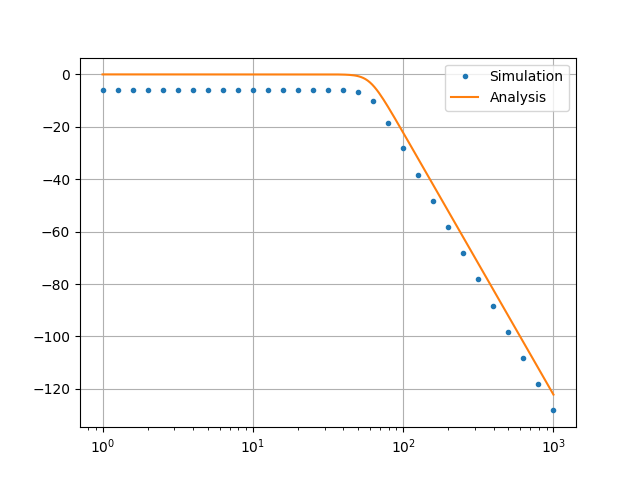
\includegraphics[width=\columnwidth]{figs/5_3.png}
    \caption{Simulation of Butterworth filter.}
    \label{fig:sim-butter}
\end{figure}
\solution Looking at the table of normalized element values
of the Chebyshev filter for order 3 and 0.5 dB ripple,
and de-nomrmalizing those values, taking $f_c = \SI[parse-numbers=false]{50}{\hertz}$,
\begin{align}
    C_1' = \SI{4.43}{\milli\farad} \\
    L_2' = \SI{3.16}{\milli\henry} \\
    C_3' = \SI{6.28}{\milli\farad} \\
    L_4' = \SI{2.23}{\milli\henry}
\end{align}
The L-C network is shown in Fig. \ref{fig:cheby-filter}.

\begin{figure}[!ht]
    \centering
    \begin{circuitikz} 
        \draw (0,0) to[short, o-o] (7,0); 
        \draw (1,0) to[C, l=4.43 mF] (1,2);
        \draw (3.5,0) to[C, l=6.28 mF] (3.5,2);
        \draw (0,2) to [short, o-] (1,2) to [L, l=3.16 mH] (3.5,2) to[L, l=2.23 mH] (6,2) to[short, -o] (7,2);
    \end{circuitikz}
    \caption{L-C Chebyshev Filter}
    \label{fig:cheby-filter}
\end{figure}

This circuit is simulated in the ngspice code \texttt{codes/5\_4.cir}.
The Python code \texttt{codes/5\_4.py} compares the amplitude response
of the simulated circuit with the theoretical expression.
\begin{figure}
    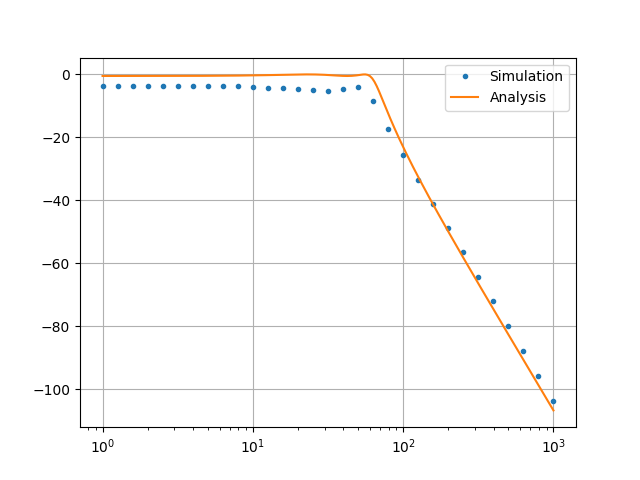
\includegraphics[width=\columnwidth]{figs/5_4.png}
    \caption{Simulation of Chebyshev filter.}
    \label{fig:sim-cheby}
\end{figure}

\item Design a low pass digital Butterworth filter for your $H(f)$.

\solution 

\item Design a low pass digital Chebyshev filter for your $H(f)$.

\solution
\end{enumerate}
\end{document}
